%!TEX encoding = IsoLatin

%
% Chapitre "Architecture"
%

\chapter{Architecture}

Paint3D+ est organis�e en plusieurs classes qui supportent ces fonctionnalit�s. La structure 
hi�rarchique permet de minimaliser le volume du code n�cessaire et de faciliter l'impl�mentation de plusieurs fonctions (comme les transformations interactives, la s�lection multiple, etc.). Comme le programme fonctionne en 3 mods diff�rents, on peut grouper les classes en 3 parties respectivement: les classes qui supportent le mode 2D, le mode 3D et la partie du rendu qui est construite autour de la casse ''OfApp'' (fournie initialement par Openframworks).
\\

La vue d'ensemble est repr�sent�e dans la figure suivante:

\begin{figure}[h] 
\begin{center}
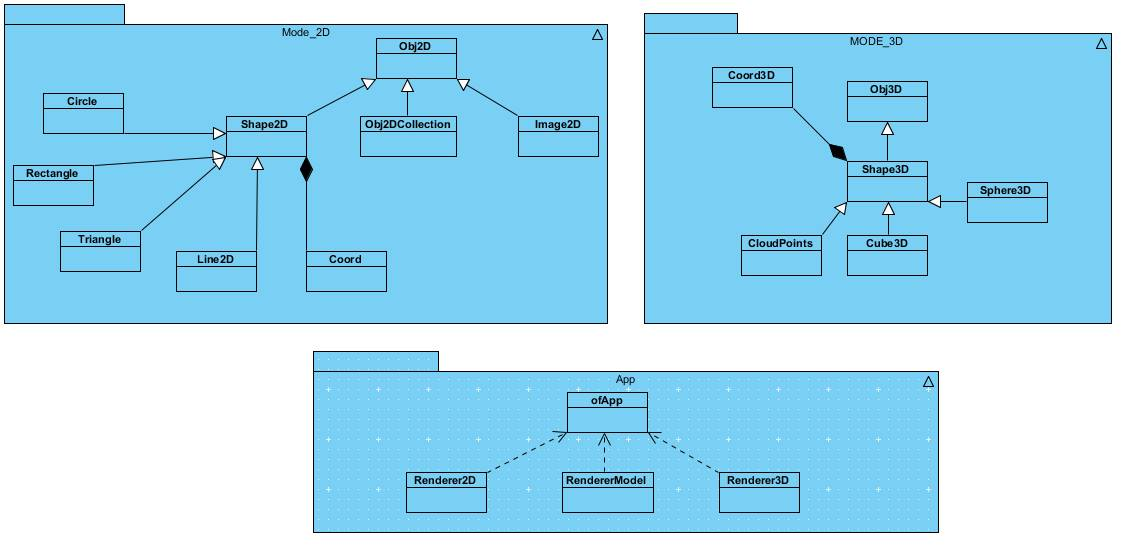
\includegraphics[width=15cm, height=10cm]{fig/uml1.jpg}
\end{center}
\caption{Diagramme UML vue d'ensemble.}
\end{figure}

Les d�tails pertinents de chaque classe sont pr�sents dans les diagrammes suivants:

\newpage

\begin{figure}[h] 
\begin{center}
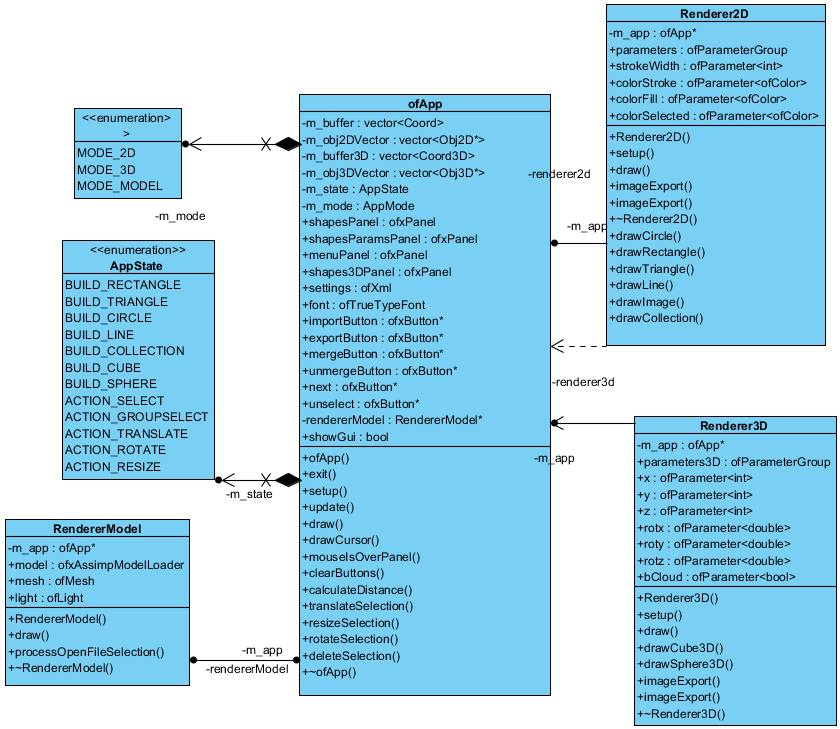
\includegraphics[width=15cm, height=10cm]{fig/uml2.jpg}
\end{center}
\caption{Diagramme UML de ofApp.}
\end{figure}

\begin{figure}[h] 
\begin{center}
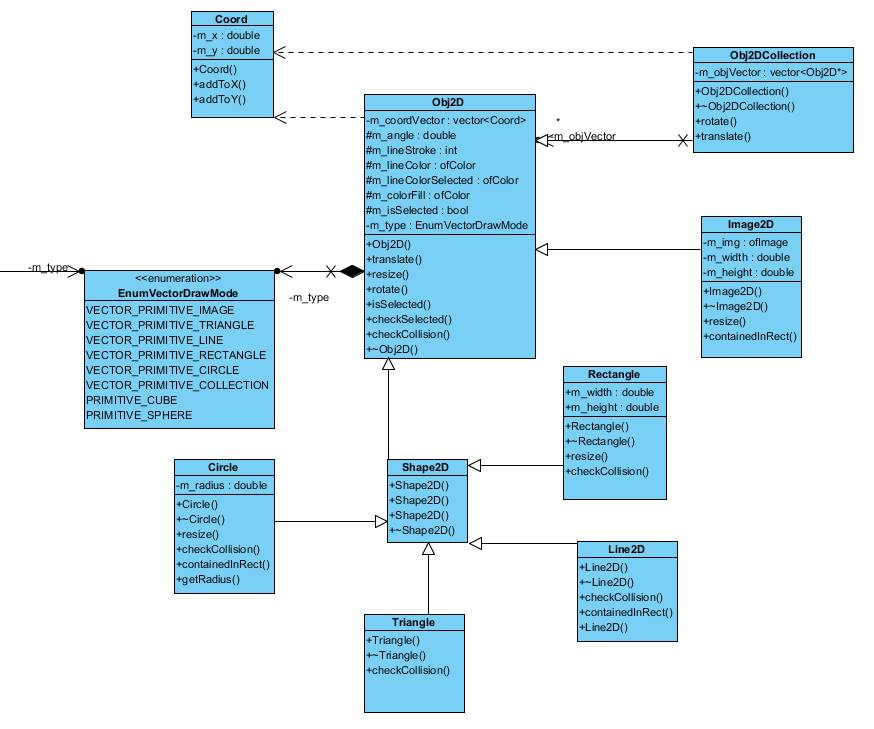
\includegraphics[width=15cm, height=10cm]{fig/uml3.jpg}
\end{center}
\caption{Diagramme UML du 2D.}
\end{figure}

\begin{figure}[h] 
\begin{center}
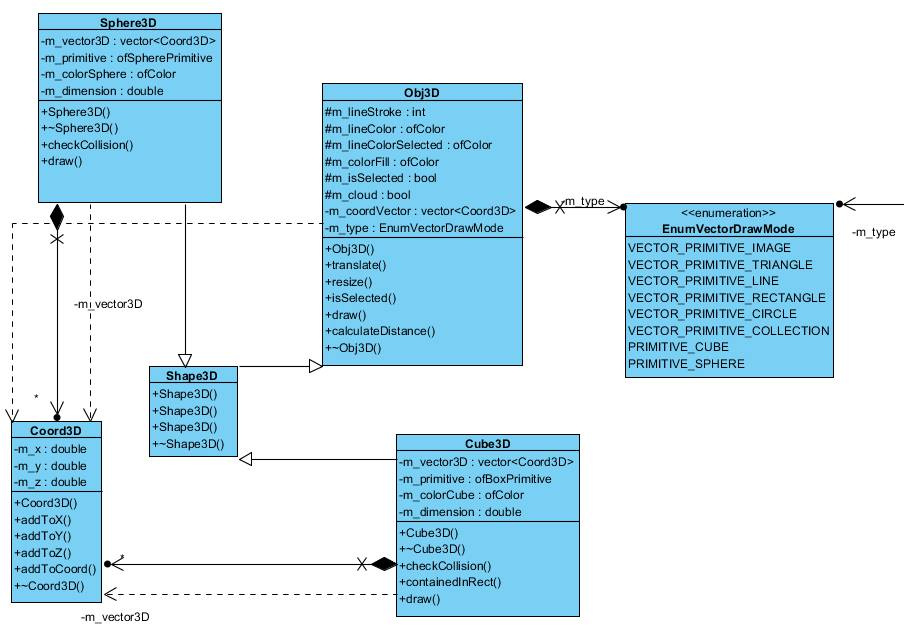
\includegraphics[width=15cm, height=10cm]{fig/uml4.jpg}
\end{center}
\caption{Diagramme UML du 3D.}
\end{figure}

\newpage 

Il faut tenir compte que le r�le de ces diagrammes est de montrer l'architecteur de l'application et la logique de fonctionnement (par exemple les m�thodes ''set'' et "get')' ont �t� omises pour simplifier la complexit� des diagrammes. Pour plus de d�tails, il faut consulter leur impl�mentation (le code dans les fichier .h et .cpp respectivement).